\section{Background}            
The field of virtual reality (VR) technology has seen an exciting development in recent years, 
with the release of the first commercial virtual reality headsets, such as Oculus Rift CV1 and HTC Vive, taking place in 2016.

The application area for these virtual reality headset have exceeded the expectations of many, with virtual reality 
technology being present in domains ranging from entertainment to educational training\citep{VRS2016}. 
\citet{VRS2016} reports numerous domains where virtual reality is successful being used, including 
healthcare (e.g surgery), military, architecture/construction, art, fashion, entertainment (games, films etc), education, business, telecommunications, sports and rehabilitation.

Despite this early success, there are still a lot challenges associated with virtual reality technology. One of these challenges is related to human-computer interactions
and will be expanded upon later in this chapter. This chapter will first discuss the virtual reality field and how gesture recognition technology can be very relevant for it,
before defining the problem definition, limitations and outline for the rest of this thesis.
%Making good use of virtual reality comes with several challenges, which will be discussed later. 

%Although these devices' initial target market was the games- and entertainment industry, 
%the applications of these devices in other domains have already exceeded the expectations of many~\citep{VRS2016}. 
% Examples of such domains include the military, the educational system, the healthcare industry, the construction businesses and the telecommunications industry~\citep{VRS2016}. 


\section{Virtual Technology}
Virtual reality can be defined as a realistic and immersive simulation of a three-dimensional 360 degree environment, 
created using interactive software and hardware, and experienced or controlled by movement of the body \citep{VRS2016}.
This virtual environment is perceived through a virtual reality headset, which is a stereoscopic head-mounted display (HMD) that provide separate images for each eye \citep{POLYGON2016}. 
In addition to separate eye displays a HMD typically also contains head motion sensors such as gyroscopes, accelerometers 
and other sensors to track the user's head movements\citep{TW2016}. 
A person using a virtual reality head-mounted display should thus perceive a virtual world with realistic depth vision and be able to "look around" by turning his or her head.

The development of virtual reality head-mounted displays was in many ways fueled by the development of smart phones as many of the components are similar (e.g.~gyroscopes), and
these components also became more affordable by the prominence of smart phones. 
This led to the prototype HMD "Oculus Rift Development Kit 1", released by Oculus VR in 2012, being the first independently developed and sold virtual reality headset\citep{TW2016}. 

\begin{figure}%[h!] %[H]
	\includegraphics[width=\linewidth]{pictures/oculus_rift_dk1.jpg}
	\caption[The Oculus Rift Development Kit 1]{The Oculus Rift Development Kit 1, released by Oculus VR in 2012.}
	\label{fig:oculus}
\end{figure}

As virtual reality technology enables users to experience virtual worlds in a new way, 
human-computer interaction (HCI) is also a highly relevant topic. 
This field has in many ways seen a resurgence as virtual technology gives new possibilities, but also set new constrains. 
One of these constraints is limiting the user's field of vision exclusively to that projected by the lenses, 
which may make interaction with traditional input devices, such as mouse and keyboard, more challenging. 
Because of this, alternate methods of interacting with the computer is a relevant topic. 
One of these methods is the use of gestures, 
which have long been considered an interaction technique that can potentially deliver more natural, 
creative and intuitive methods for communicating with our computers~\citep{Rautaray2015}. 
To enable the use of gestures as a viable input method to a computer, responsive and reliable gesture recognition techniques are needed.  

\section{Gesture Recognition Technology}
A gesture can be defined as a physical movement of the hands, arms, face and body with the intent to convey information or meaning~\citep{Mitra2007}, 
Even though the use of keyboard and mouse is a prominent interaction method, there are situations in which
these devices are impractical for human-computer interaction (HCI). This is particularly the case for interaction with 3D objects~\citep{Rautaray2015}. 

To be able to convey semantically meaningful commands through the use of gestures one must rely on a gesture recognition system, 
which is responsible for capturing and interpreting gestures from the user and, if applicable, carry out the desired action. 
Often this process is seen as a sum of three fundamental phases: Detection, tracking and recognition~\citep{Rautaray2015}.

\subsection{Detection}
The first step in a typical gesture recognition system is to detect the relevant parts of the captured image and segment them from the rest. 
This segmentation is crucial because it isolates the relevant parts of the image from the background to ensure that only the relevant part is processed by the subsequent 
tracking and recognition stages~\citep{Cote2006}. 
A gesture recognition system will typically be interested in hand gestures, head- and arm movements and body poses, and thus only these factors should be observed by the system.

\subsection{Tracking}
The second step in a gesture recognition system is to track the movements of the relevant segments of the frames, e.g.~the hands. 
Tracking can be described as the frame-to-frame correspondence of the segmented hand regions and aims to understand the observed hand movements. 
This is often a difficult task as hands can move very fast and their appearance can change vastly within a few frames, 
especially when light condition is a big factor~\citep{Wang2010}. 
One additional note is that if the detection method used is fast enough to operate at image acquisition frame rate, it can also be used for tracking~\citep{Rautaray2015}.   

\subsection{Recognition}
The last step of a gesture recognition system is to detect when a gesture occurs. 
This often implies checking against a predefined set of gestures, each entailing a specific action. 
To detect static gestures (i.e postures involving no movement) a general classifier or template-matcher can be used, 
but with dynamic gestures (which involves movement) other methods, which keep the temporal aspect, such as a Hidden Markov Model (HMM), are often required~\citep{Benton1995}. 
The recognition technology often makes uses of several methods from the field of machine learning, including supervised, unsupervised and reinforced learning.

When a gesture recognition system detects a relevant segment, it is thus tracked and represented in some way in the system. For hand gesture representations, 
which is the most relevant for this thesis, there are two major categories of hand gesture representations: 3D model-based methods and appearance-based methods~\citep{Rautaray2015}.

\begin{figure}%[h!] %[H]
	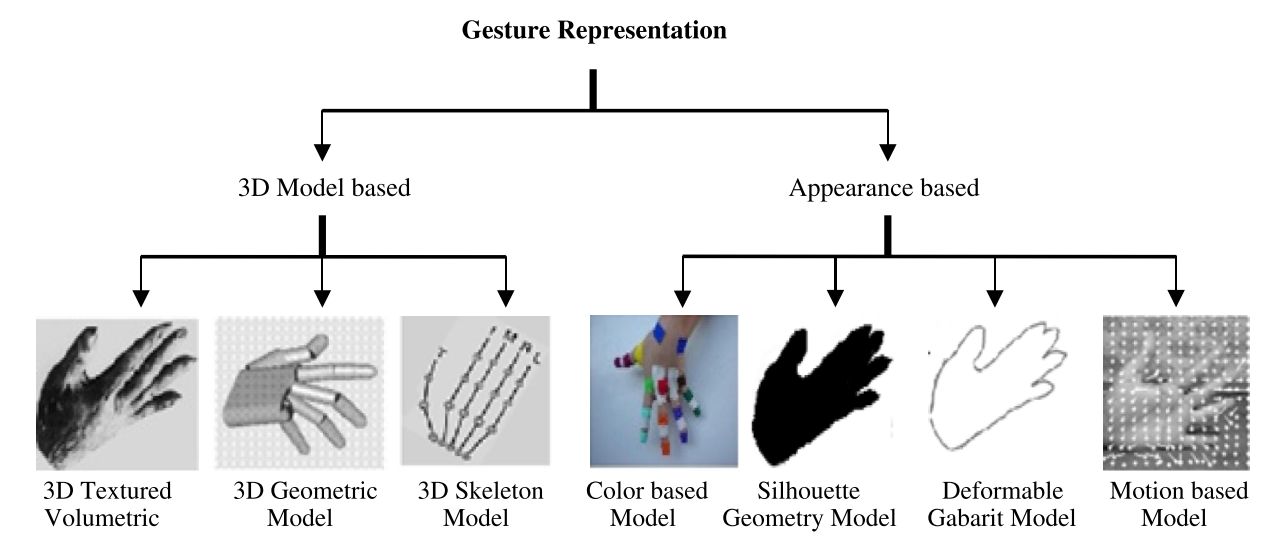
\includegraphics[width=\linewidth]{pictures/gesture_representation.png}
	\caption[Vision-based hand gesture representations]{Vision-based hand gesture representations~\citep{Bourke2007} }
	\label{fig:oculus}
\end{figure}


\section{Problem definition}
%This thesis will explore the possibilities of utilizing virtual reality- and gesture recognition technology in combination 
%during the design review process of the major international classification company DNV GL. 
%This will be accomplished by implementing a design review application that makes use of both these technologies for several design review tasks (see section 2.1), 
%and by having users evaluate the effectiveness of these techniques. 
%This essay will summarize DNV GL's design review process, list the application requirements, 
%discuss some of the developments within the field of gesture recognition technology and briefly review the Leap Motion Controller.


This thesis will evaluate the consequences of utilizing virtual reality technology in combination with vision based gesture recognition technology, and discuss the benefits it 
might bring, as well and the challenges it presents. 
The thesis will also review the design and implementation of a design review application, which is developed as part of this thesis with the aforementioned goal in mind. 
The design review application is also a prototype developed for the major international classification company DNV GL to evaluate how the use of virtual reality and gesture
recognition technology might benefit their design review process. As such, the application requirements has been created in cooperation with DNV GL and represents
common 3D object manipulating and navigation tasks. After discussing the design and implementation choices of this application, the user evaluation session will be discussed. 
This user evaluation sessions where performed by DNV GL employees, and potential end users, and contained invaluable feedback relevant to the use of virtual reality and gesture
recognition technology in a professional setting. 

\section{Limitations}
The initial list of application features had to be shortened significantly to focus more on the most relevant parts for this thesis. As such the design review application
is more a prototype or proof-of-concept than a finished product. Section X outlines the application features and will explain more of whats include in the application and what isn't. 

\section{Outline}
This thesis is organized as follows: In chapter 2 we will review the history and theoretical foundations for virtual reality and gesture recognition technology, as well
as discuss some of their primary challenges. In chapter 3 we will review the design of the design review application, and how the applications defines and detect gestures. 
Chapter 4 will go more into the technical details of how the application is implemented and serve as a documentation for the source code.
In chapter 5 the user trials will be covered, and the responses discussed and analyzed.
Chapter 6 concludes the thesis with a quick summary, some thoughts about future work and a conclusion.

